\chapter{Metodologia}\label{cap:metodologia}

Uma vez introduzidos à temática deste trabalho graduação, seu objetivo e os principais conceitos que o circundam, é possível agora abordar as etapas percorridas para executá-lo e, eventualmente, possibilitar que outros, iniciantes no estudo de aplicações de detecção e reconhecimento de texto, consigam reproduzi-lo, provendo uma documentação detalhada do caminho tomado durante o desenvolvimento do trabalho.

Sob ótica de todo o ciclo de desenvolvimento deste trabalho de graduação, houveram quatro grande marcos que servirão para estruturar esse capítulo:

\begin{enumerate}
    \item Experimentação com soluções de reconhecimento e detecção de texto.
    \item Desenvolvimento da solução fim-a-fim a partir de detectores e reconhecedores de texto.
    \item Avaliação da solução fim-a-fim proposta.
    \item Publicação da solução em ambientes de computação em nuvem.
\end{enumerate}

1. Experimentação com soluções de reconhecimento e detecção de texto
2. Desenvolvimento da solução fim-a-fim a partir de detectores e reconhecedores de texto
3. Avaliação da solução fim-a-fim proposta
4. Publicação da solução em ambientes de computação em nuvem

Dessa forma, as sub-seções a seguir detalharão cada uma dessas etapas, sob perspectiva da experiencia do autor durante a execução deste trabalho de graduação.

\section{Experimentação com soluções de reconhecimento e detecção de texto}\label{sec:metodologia_experimentacao}

Apesar de já ter sido mencionado a escolha dos componentes de detecção, CRAFT, e de reconhecimento, CRNN, não foi abordado o processo adotado que culminou nessa escolha. Nessa seção será abordado um pouco da motivação sobre essas escolhas, sob caráter mais técnico e pratico sobre as soluções públicas, que são de fácil acesso através da internet. 

A partir de uma rápida busca na internet, em especial na plataforma do GitHub, hospedeiro de repositórios de código fonte versionados pela ferramenta Git, famoso sistema controlador de versão, é possível encontrar diversos repositórios mencionando soluções para detecção e reconhecimento de texto em cenas, as vezes até mesmo repositórios oficiais, oferecidos pelos autores de trabalhos famosos na área, como é o próprio exemplo do detector de texto CRAFT.

No entanto, uma grande dificuldade para de fato conseguir executar o código desses repositórios é satisfazer os requisitos e dependências minímas, muitas vezes implícitos, por exemplo, a obrigatoriedade de possuir hardware com placa gráfica compatível com a versão utilizada no momento de desenvolvimento do trabalho original, a indisponibilidade dos modelos pré-treinados para rápida verificação de resultados, a base de código incompleta, sem todas as instruções para execução ou com dependências de versões antigas de linguagem de programação, bibliotecas e/ou frameworks, entre outros.

Um outro ponto de grande valor na escolha dos métodos aplicados neste trabalho é a compatibilidade entre os métodos de detecção e reconhecimento. Como o grande objetivo deste trabalho se baseia na integração dessas soluções para que trabalhem juntas, o caminho mais simples nessa linha é que ambos projetos consigam se executados dentro do mesmo ambiente de desenvolvimento, com dependências em bibliotecas e frameworks parecidos, se não, iguais, para que não houvessem conflitos entre ambos os projetos que trouxessem problemas em tempo de execução.

Na escolha do método de detecção de texto, a partir de uma revisão de trabalhos anteriores da área, foi considerado e, até certo ponto, experimentado, códigos oficiais e re-implementações publicas dos seguintes trabalhos:

{{TODO: listas trabalhos e repositórios}}

Por fim, o que foi mais acessível em relação aos pontos citados anteriormente foi o código-fonte do CRAFT. Os autores desenvolveram o modelo em Python, usando o framework PyTorch, que é bastante difundido, o que facilita na escolha de projetos para integrar o reconhecimento de texto. Os autores também disponibilizaram os modelos pré-treinados para detecção de texto em cenas, o que é um grande diferencial, já que o procedimento de treinamento dessas soluções não são triviais, além de costumarem ser bastante custosos temporal e computacionalmente, o que desviaria o foco do objetivo desse trabalho. Adicionalmente, o código fonte contém instruções minímas de como executar o modelo pré-treinado, que se mostraram suficientes para iniciantes sem muita experiencia prévia com a linguagem de programação e em trabalhos de detecção de texto. Outro diferencial foi a possibilidade de executar o modelo pré-treinado em hardwares sem aceleração gráfica, mesmo que com a penalização no tempo de execução, já que os componentes compatíveis não são baratos, em no contexto atual de cripto moedas e escassez de chips gráficos no mercado.

Agora sobre a escolha do método de reconhecimento, como já temos que o detector escolhido usa a linguagem Python e o framework PyTorch, filtramos os métodos disponíveis por esses critérios. Uma implementação do CRNN em PyTorch foi escolhida pois atendia os critérios de compatibilidade com a linguagem, framework e bibliotecas que o CRAFT depende aliado ao fato do CRNN ser uma solução bastante popular, com implementação bastante sucinta e, novamente, de fácil execução a partir de um modelo pré-treinado, o que também foi fornecido pelo autor da implementação.

{{ TODO: 
- Explicar como executar cada um?
- Explicar a parametrização de cada um? Inputs e Outputs?
- Explicar }}

A próxima sub-seção abordará, com um pouco mais de detalhes, como as duas soluções escolhidas foram integradas em uma mesma base de código e como os resultados do CRAFT foram processados para que pudessem alimentar a implementação do CRNN, completando a solução fim-a-fim do reconhecimento de texto. 

\subsection{Desenvolvimento da solução fim-a-fim a partir de detectores e reconhecedores de texto}\label{sec:metodologia_desenvolvimento}

A fim de aplicar o reconhecimento, utilizando o CRNN, exatamente sobre o texto detectado e localizado pelo CRAFT, a escolha foi utilizar o repositório com o código fonte do detector CRAFT como base inicial para a aplicação de reconhecimento fim-a-fim e, a partir dele, adicionar a solução de reconhecimento dentro da mesma base de código e fazer com que ambas tenham todas as dependências necessárias para conseguirem executar seu processamento. Em outras palavras, foi necessário preparar um ambiente de desenvolvimento Python todas a dependências, a nível de linguagem de programação, bibliotecas e frameworks, instalados e sem conflitos, com tanto as bibliotecas que são dependências obrigatórias para a implementação do CRAFT quanto as bibliotecas que são utilizadas na implementação do CRNN.

Para a gestão de ambientes de desenvolvimento e suas dependências, foi utilizado uma ferramenta no ecossistema Python chamada Conda, mantida pela empresa Anaconda. Com essa ferramenta é possível criar ambientes virtuais Python e instalar todas as dependências necessárias dentro desses ambientes virtuais usando poucas instruções na linha de comando do computador. A própria ferramenta fornece meios para de gerir os ambientes virtuais criados e otimiza a instalação de pacotes dentro desses ambientes de forma que conflitos sejam evitados, resolvendo as versões dos pacotes instalados de forma que sejam compatíveis entre si e compatíveis com a versão da linguagem Python escolhida para o ambiente. Uma grande vantagem de usar esse gerenciados de ambientes Python é a possibilidade de reproduzir qualquer ambiente previamente configurado a partir de um arquivo de configuração, do tipo YAML, que lista todos os pacotes instalados em um ambiente virtual para que, a partir desse arquivo, a ferramenta consiga remontar o mesmo ambiente sem precisar de configurações manuais novamente.

Entrando mais no caminho percorrido para integrar as duas soluções, o primeiro passo foi replicar os repositórios para a conta pessoal do autor no GitHub. Esse processo dentro da plataforma se chama `fork`  e em geral é bastante utilizado para possibilitar que outras pessoas consigam desenvolver coisas novas na base de código sem ter o risco de empurrar mudanças no repositório original inadvertidamente. Dessa forma, ambos os repositórios foram replicados para a conta pessoal do autor e todo o desenvolvimento deste trabalho foi feito nos repositórios replicados.

A partir dos repositórios replicados, foi utilizado um recurso da ferramenta de versionamento, o Git, que possibilita a composição de repositórios a fim de facilitar a sincronização das bases de códigos. O recurso em questão é a criação de sub-módulos em um repositório Git. Usando o comando abaixo a partir do repositório replicado do detector, foi gerado um relacionamento entre as duas bases de código, sendo que o repositório do CRNN agora é visto como um sub-modulo do repositório do CRAFT, e, a partir disso, é possível baixar, usar, evoluir a base de código do repositório do CRNN diretamente do repositório do CRAFT. Isso fez com que ambas soluções já tenham visibilidade uma da outra, mas ainda faz com que trabalhem juntas.

```console
git submodule add https://github.com/mmilani1/crnn.pytorch
```

Com as soluções na mesma base de código, uma etapa importante é a garantir que ambas ainda funcionam de forma isolada e se validar a compatibilidade das dependências de cada uma. Como mencionado na Seção \ref{sec:metodologia_experimentacao}, uma das motivações da escolha especificamente dessas duas implementações citadas foi justamente a maior proximidade em termos de frameworks e bibliotecas que utilizam, inclusive a possibilidade de ambas soluções poderem ser executadas sem a necessidade de aceleração gráfica. Dessa forma não houveram problemas em executar separadamente cada solução, mesmo compartilhando o mesmo ambiente virtual. O arquivo YAML com a descrição do ambiente virtual pode ser consultado diretamente do repositório com a implementação ou no Apêndice \ref{apd:yaml-desenvolvimento}.

A partir deste ponto já se torna possível trabalhar com os modelos de detecção e reconhecimento a fim de integrá-los, de alguma forma. O objetivo ao fim da integração é conseguir reconhecer texto em imagens de cena, para isso, a ideia é evoluir a extração de resultados do modelo de detecção CRAFT para gerar uma lista de recortes das regiões de texto da imagem original e implementar um algoritmo que execute o modelo de reconhecimento CRNN para cada um desses recortes.

Conforme detalhado na Seção \ref{sec:metodologia_experimentacao}, a implementação do CRAFT fornecida é didática o suficiente com os resultados da detecção, gerando visualizações dos resultados junto com um arquivo de texto contendo as coordenadas das regiões de texto detectadas. Isso demonstra que, em algum ponto do código original as coordenadas dessas regiões de texto foram manuseadas pelos autores do modelo e, consequentemente, poderão ser manuseadas no desenvolvimento da solução integrada a fim de gerar os recortes que serão posteriormente consumidos pelo modelo reconhecimento. O Algoritmo \ref{alg:pseudo_codigo} apresenta o pseudo-algoritmo com as etapas do processamento executado.


\begin{algorithm}
\caption{Pseudo-Código da integração entre a detecção e o reconhecimento de texto}\label{alg:pseudo_codigo}
\begin{algorithmic}
\State $imagem \gets{lerEntrada()}$
\State $palavras \gets{[ ]}$
\State $regioesDeTexto \gets{executaDeteccaoCRAFT(imagem)}$
\For{$regiaoDeTexto \in regioesDeTexto$}
    \State $recorte \gets{recortarTextoDaImagemOriginal(imagem,regiaoDeTexto)}$
    \State $palavra \gets{executaReconhecimentoCRNN(recorte)}$
    \State $palavras \gets{paralvras + [palavras]}$
\EndFor
\State{}
\Return{$palavras$}
\end{algorithmic}
\end{algorithm}

% ```
% imagem = lerEntrada()
% vetoreDePalavrasReconhecidas = []
% vetorDeRegioesDeTexto = detectorCRAFT(imagem)

% para cada regiao em vetorDeRegioesDeTexto:
%   regiaoDeTextoExtraida = extrairRegiaoDaImagemOriginal(regiao)
%   palavra = reconhecimentoCRNN(regiãoDeTextoExtraida)
%   vetorDePalavrasReconhecidas << palavra

% retorna vetorDePalavrasReconhecidas
% ```

Para efetuar o recorte das regiões de texto localizadas e fornecidas na saída do modelo de detecção, foi utilizado um par de funções da biblioteca OpenCV, especializada em ferramentas voltadas para visão computacional. As funções utilizadas foram \texttt{cv2.getPerspectiveTransform} e \texttt{cv2.warpPerspective}.
A primeira função é responsável por gerar uma matriz de transformação de áreas quadrangulares e recebe duas sequencias de pontos. A primeira sequencia contém os vértices da área quadrangular a ser transformada, no caso desse trabalho, são as coordenadas da \textit{bounding-box} de uma palavra detectada. Já a segunda sequencia de pontos representa os vértices da imagem de saída, para onde o cada um dos pontos da primeira sequencia serão transportados após a aplicação da transformação.
A segunda função é responsável por aplicar a matriz de transformação, gerada a partir da execução do comando \texttt{cv2.getPerspectiveTransform}, sobre a imagem onde o texto foi detectado. Dessa forma conseguimos recortar as palavras detectadas da imagem original de forma que cada é possível posteriormente passar as referencias desses recortes para o modelo de reconhecimento diretamente, já que a os dados de entrada esperados pelo CRNN são imagens que contem idealmente uma palavra para reconhecimento. A Figura XX ilustra, em alto nível, as etapas do processamento que compõem as solução de STR fim-a-fim deste trabalho.

\begin{figure}
    \centering
    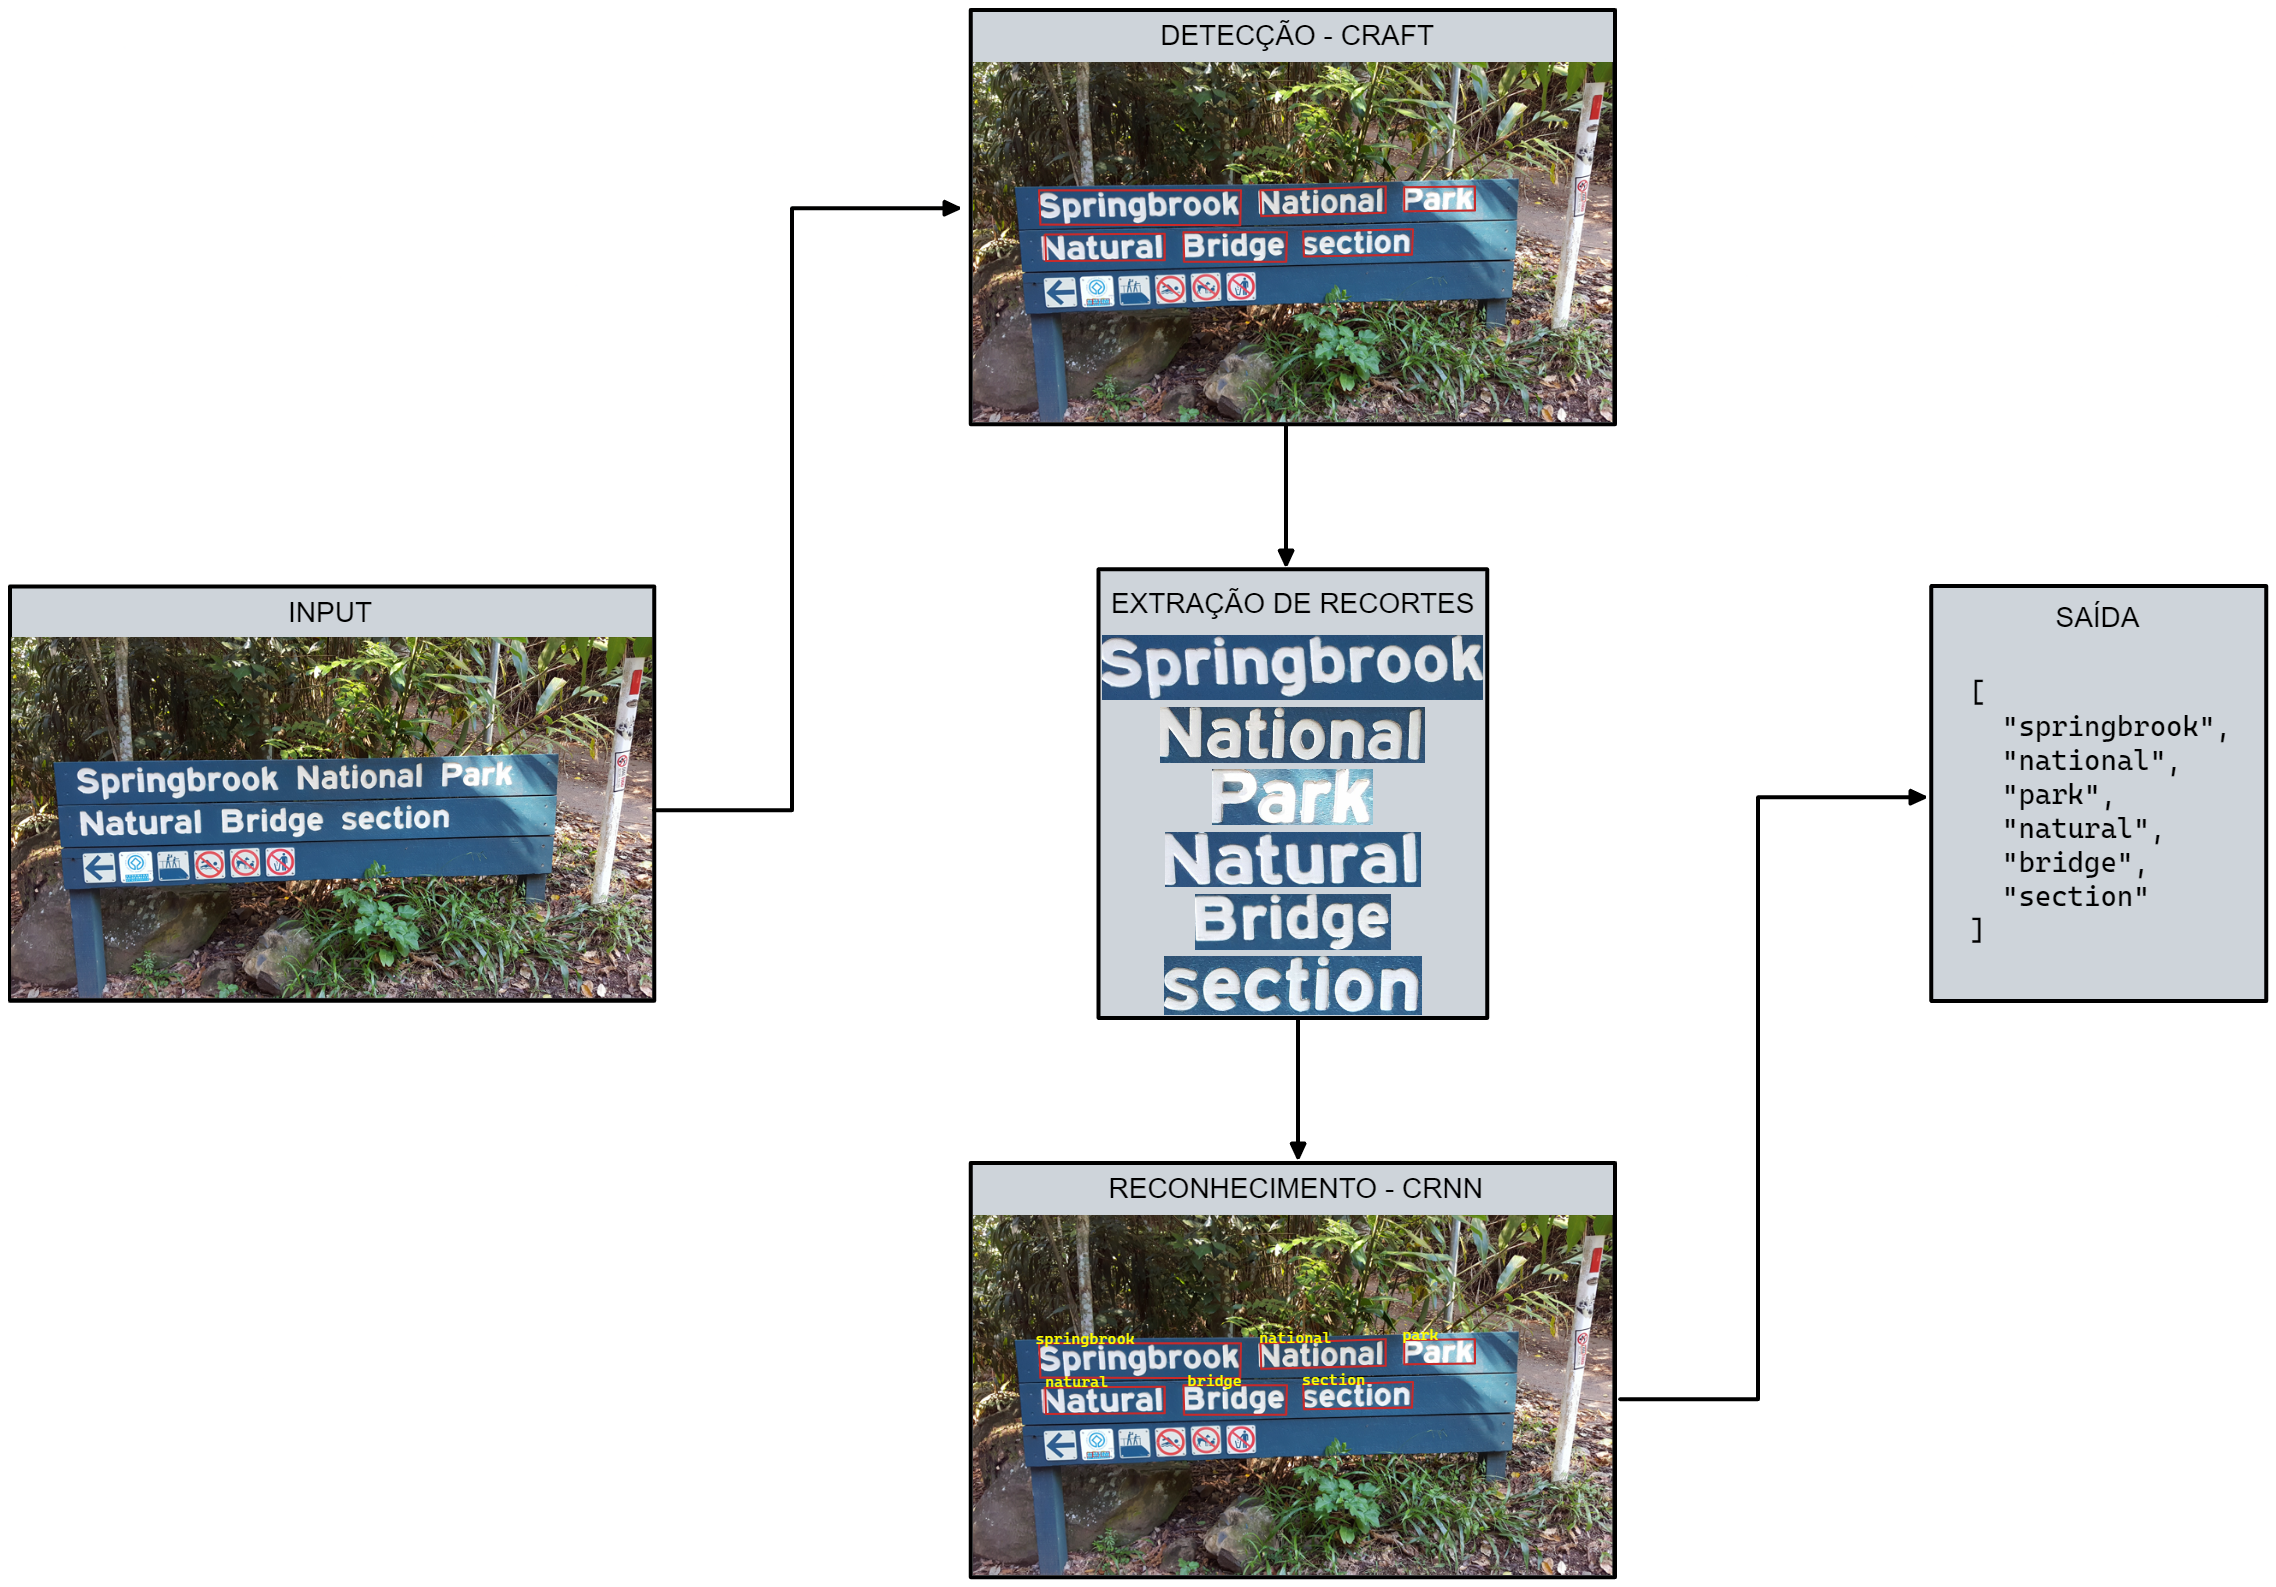
\includegraphics[width=0.8\textwidth]{figs/metodologia-pipeline.png}
    \caption{Ilustração das etapas de processamento da solução proposta. Fonte Própria}
    \label{fig:methodology_pipeline}
\end{figure}

Ao fim dessas alterações, integrando os dois modelos de detecção e reconhecimento, já temos uma solução simples de reconhecimento de texto em cenas que pode ser classificada como \textit{end-to-end}, que contempla tanto a detecção quanto o reconhecimento dentro de uma mesma aplicação. A próxima etapa é conseguir avaliar a eficácia desse novo desenvolvimento. A próxima seção introduzirá os métodos e métricas utilizadas para avaliar a solução.

\subsection{Método de avaliação da solução proposta}\label{sec:methodology_validation}

A avaliação analítica da solução proposta neste trabalho é baseada na forma de avaliação da plataforma \textit{Robust Reading Competition} (abreviação RRC), disponibilizado pelo Centro de Visão Computacional da Universidade Autônoma de Barcelona. Essa plataforma organiza competições em torno de problemas reais de visão computacional e tipicamente essas competições se relacionam com a Conferencia Internacional sobre Análise e Reconhecimento de Documentos, abreviada como ICDAR, a partir no nome da conferencia em inglês. Diversos datasets que são amplamente adotados para treino e avaliação de modelos de reconhecimento de texto levam no nome a menção ao ICDAR, por introduzirem a base da dados e os desafios propostos, fomentando novos trabalhos na área.

Essa seção irá introduzir dos datasets avaliados, as métricas utilizadas e o processo de avaliação da solução apresentada utilizando as ferramentas de avaliação disponibilizadas pela plataforma RRC.

\subsubsection{Datasets}\label{sec:methodology_datasets}

Conforme mencionado anteriormente, os datasets dos desafios vinculados ao ICDAR são muito utilizados por trabalhos voltados à detecção e reconhecimento de texto. Ambos os modelos, de detecção e de reconhecimento utilizados no desenvolvimento deste trabalho fazem referencia aos datasets ICDAR: O CRAFT cita os datasets ICDAR 2013, ICDAR 2015 e ICDAR 2017 como bases de treinamento e de validação em quanto o CRNN se refere ao ICDAR 2003 e ICDAR 2013 como bases de imagens para validação. Os datasets utilizados para a avaliação deste trabalho foram o ICDAR 2011, base para o primeiro desafio da platafoma RRC chamado Reading Text in Born-Digital Images, e o ICDAR 2013, que é a base para o segundo desafio da plataforma RRC, chamado Focused Scene Text.

\subsubsubsection{ICDAR 2011}\label{sec:datasets_icdar2011}
O ICDAR 2011 conta com 410 imagens para treino e 141 imagens para validação, imagens que estão no contexto de anúncios de internet e anexos de emails, com palavras em geral na horizontal e anotadas com bounding boxes retangulares a nível de palavras. As imagens são anotadas com a localização de cada palavra com coordenadas das bounding-boxes retangulares, que servem como gabarito para soluções de detecção e localização. Cada imagem também conta com a transição das palavras para servir como gabarito de soluções de reconhecimento conta A Figura XX expõe algumas imagens deste dataset.

\subsubsubsection{ICDAR 2013}\label{sec:datasets_icdar2013}
O ICDAR 2013 conta com 219 imagens para treino e 233 imagens para validação . São imagens de cenas onde em geral o texto tem boa qualidade e está em destaque, na orientação horizontal. As anotações de gabarito são retangulares a nível de palavras e contam com a transição das mesmas, de forma similar às imagens do ICDAR 2011. A Figura XX expõe algumas imagens deste dataset.

\subsection{Métricas}\label{sec:methodology_metrics}
Em conjunto aos datasets, são fornecidas meios de avaliação para que cada nova solução que surgir possam ser avaliadas sob os mesmos termos, usando os mesmos conceitos e as mesmas métricas. Na plataforma RCC e nos datasets que eles disponibilizam são utilizados: Precisão, Recall e F1-Score (ou H-Mean). A Precisão é a relação dos acertos (verdadeiros positivos) sobre a contagem total de predições positivas (verdadeiros positivos e falsos negativos), ou seja, dentre as predições da solução, qual é a porcentagem de acerto. O Recall relaciona a quantidade de acertos com a quantidade total de casos verdadeiros. O F1-Score é basicamente a média harmônica das métricas Precisão e Recall.

\begin{equation}
    Precisão = \frac{VP}{VP + FP}
\end{equation}
\begin{equation}
    Recall = \frac{VP}{VP + FN}
\end{equation}
\begin{equation}
    F1Score = 2 \times \frac{Precisão \times Recall}{Precisão + Recall}
\end{equation}

Para determinar se uma predição foi correta existem duas condições: A região de texto detectada deve satisfazer uma métrica característica de eficácia em detecção e localização das palavras na imagem chamada IoU, abreviação para \textit{Intersection over Union}, além da transição predita ser exatamente igual ao esperado, de acordo com as anotações do dataset. Para uma predição ser considerada correta, o valor de IoU, que se resume à precisão da detecção, deve ser maior ou igual a 50\%.

A métrica de IoU pode ser calculada a partir das coordenadas verdadeiras de uma região de texto, documentadas nas anotações dos datasets, e das coordenadas preditas pelo modelo de detecção. Ambos conjuntos de coordenadas descrevem uma área retangular para os dois datasets utilizados. Com esses dois conjuntos de valores, pode-se avaliar tanto o tamanho da intersecção entre a área predita e a área esperada, quanto o tamanho da união entre ambas as áreas. O valor numérico da métrica IoU decorre, conforme sugerido pelo nome da métrica, da divisão entre o tamanho da intersecção sobre o tamanho da união entre as áreas preditas e as áreas esperadas.

\subsection{Interface de Validação}\label{sec:methodology_validation_interface}
Na plataforma do RRC é possível avaliar uma solução formalizando a submissão dos resultados diretamente no site da competição, dessa forma os resultados ficam registrados na plataforma e pode ser até ranqueada junto a outros trabalhos submetidos. Para cada desafio existe o ranque de soluções, onde é pode-se observar resultados de outros trabalhos de maneira simple e, quando disponível, até consultar quem foram os autores, se existe algum repositório publico para a base de código, visualizar o artigo do trabalho, etc.

No entanto não é a única opção. Também existe a opção de efetuar o download dos scripts que calculam os resultados, nos mesmos moldes da avaliação remota, a fim de executar todo o processo localmente, o que foi o método adotado para esse trabalho.

Para ambos os meios de validação, é necessário preparar arquivos de resultados, para cada imagem do dataset de validação, com os dados necessários para a avaliação. Tanto o ICDAR 2011 quanto o ICDAR 2013 demandam arquivos com o mesmo formato, que se assemelham justamente aos arquivos de gabarito dessas bases, e seguem o seguinte formato:

\begin{itemize}
    \item É necessário gerar um arquivo de texto, para cada imagem, nomeados respeitando o seguinte formato: \texttt{res\_img\_\#.txt}, onde o \texttt{\#} corresponde ao identificador numérico da imagem no dataset.
    \item Cada arquivo deve ter uma linha para cada palavra detectada e reconhecida.
    \item Cada linha deve conter os seguintes valores, separados por virgula simples, exatamente na ordem especificada: posição do vértice esquerdo superior da bounding-box, vértice direto inferior da bounding-box e texto da transição.
\end{itemize}

Após gerar todos os arquivos necessários, resta submeter a agregá-los em um arquivo comprimido do tipo ZIP e, ou submeter a solução diretamente na plataforma da competição, ou executar a ferramenta de validação localmente. Os arquivos de execução local são escritos em Python de dependem de poucas bibliotecas, e executa um leve servidor web para servir a aplicação de validação. Durante a execução da validação deste trabalho, foi utilizado novamente a ferramenta Conda para gerir essas dependências. O Apêndice \ref{apd:yaml-validacao} contém o arquivo que descreve o ambiente virtual utilizado. A Figura \ref{fig:methodology_validation_interface} mostra um pouco da interface de usuário que a a aplicação fornece, com as funcionalidades de submeter o arquivo comprimido de solução e a Figura \ref{fig:methodology_validation_interface_details} mostra a funcionalidade de verificação dos resultados sobre cada imagem, possibilitando a análise sobre onde as soluções funcionaram bem e onde não funcionaram tão bem, o que foi feito no contexto da solução proposta nesse trabalho no Capitulo \ref{cap:resultados}.

\begin{figure}
    \centering
    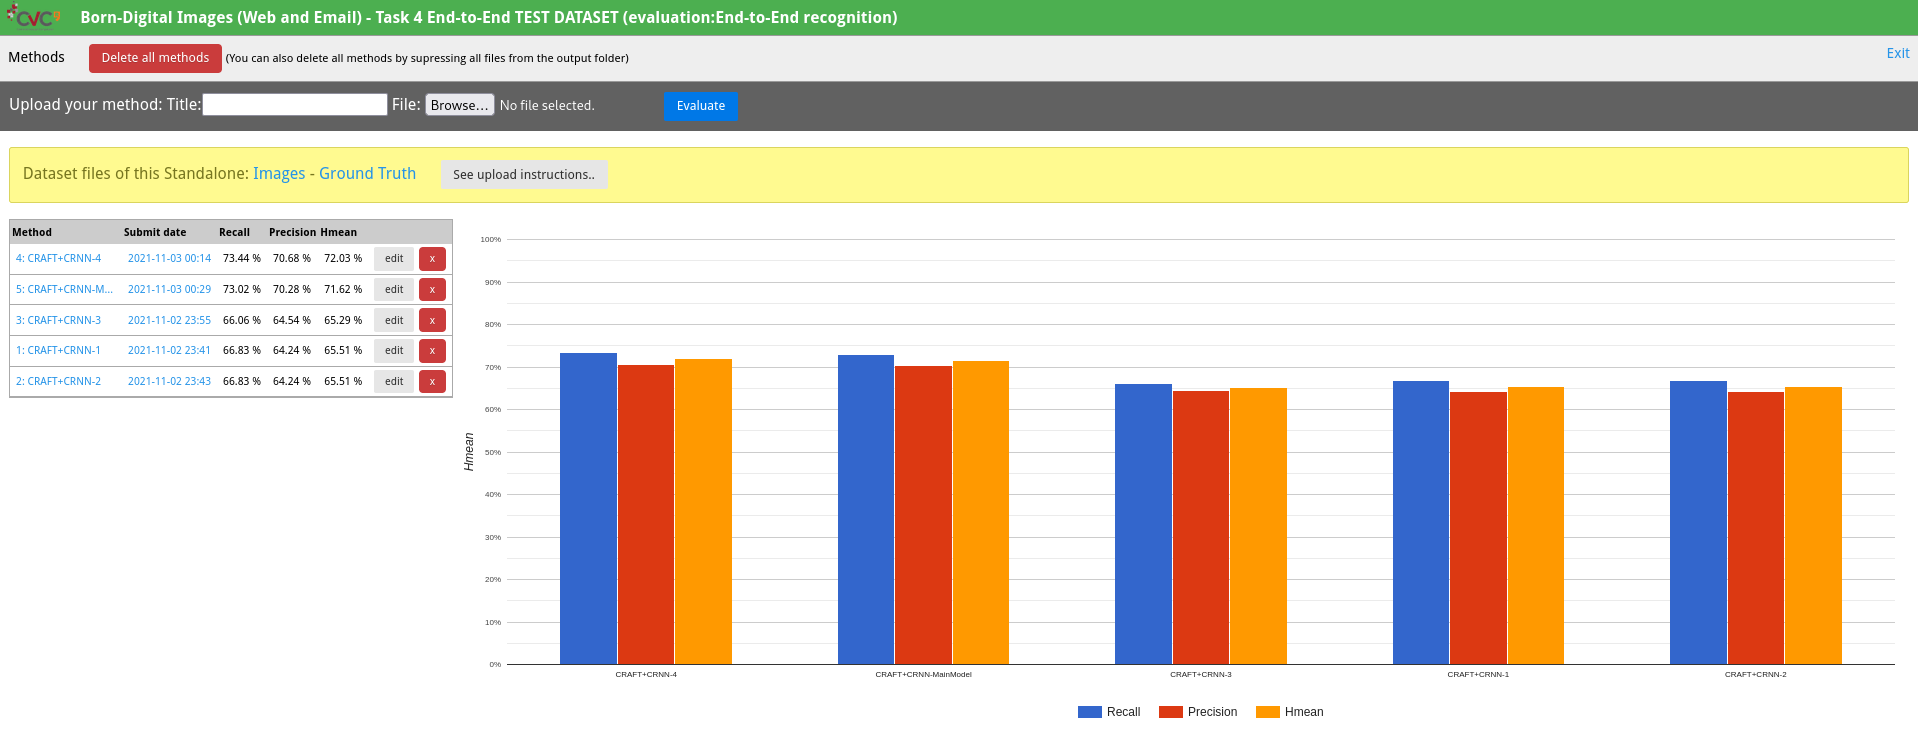
\includegraphics[width=0.8\textwidth]{figs/metodologia-interface-validacao.png}
    \caption{Interface de validação disponibilizada pela plataforma de desafios Robust Reading Competition. Fonte Própria}
    \label{fig:methodology_validation_interface}
\end{figure}

\begin{figure}
    \centering
    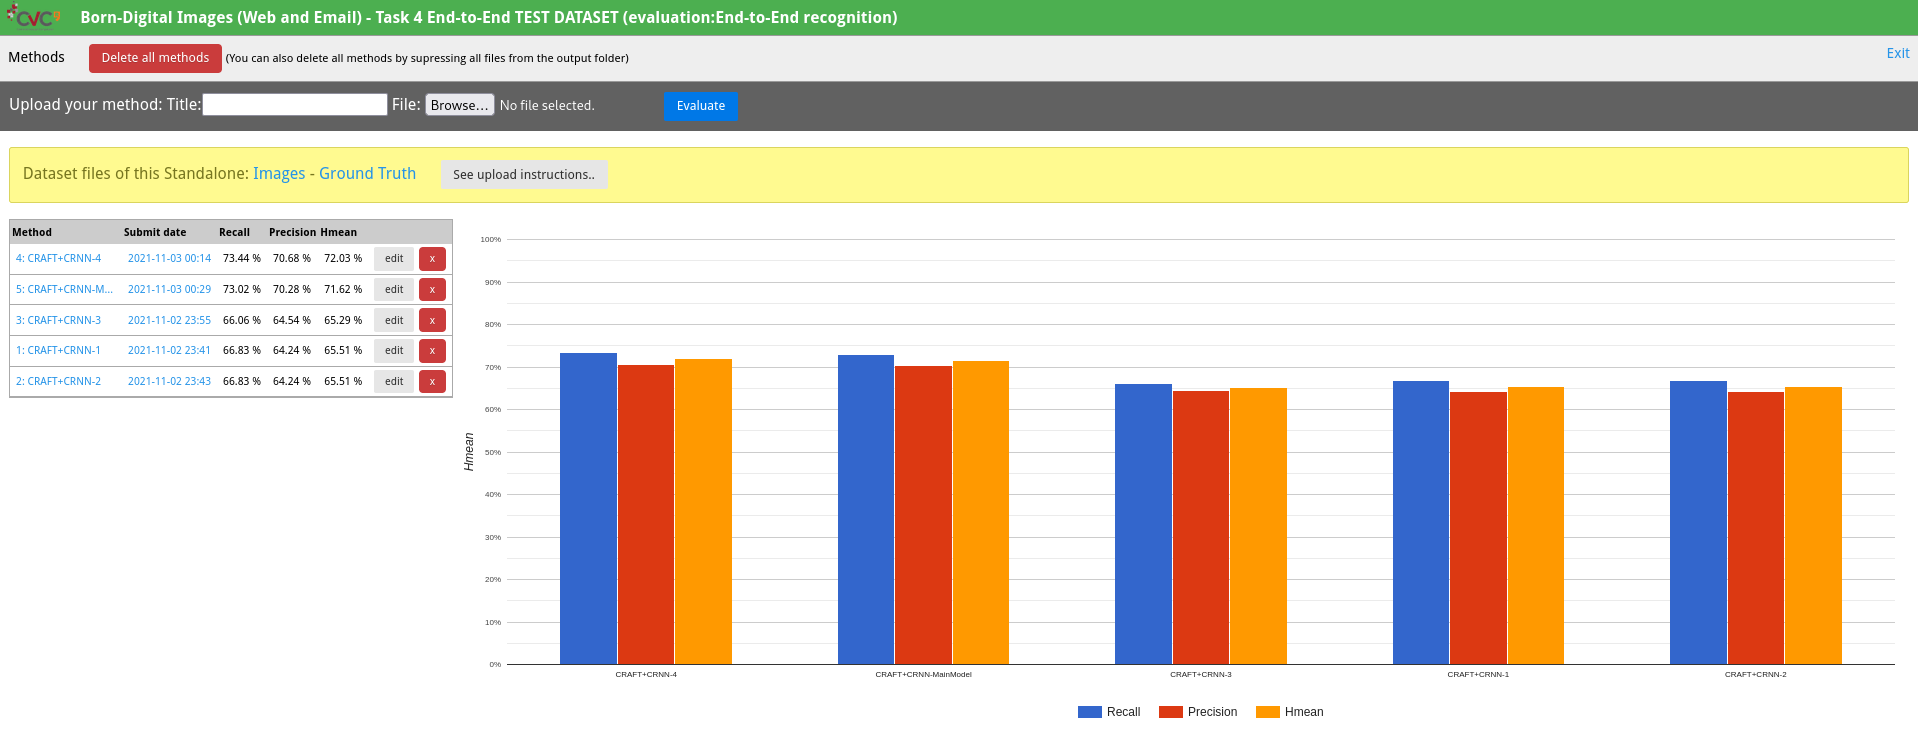
\includegraphics[width=0.8\textwidth]{figs/metodologia-interface-validacao.png}
    \caption{Interface de validação disponibilizada pela plataforma de desafios Robust Reading Competition, com visualização de detalhes da avaliação por imagem. Fonte Própria}
    \label{fig:methodology_validation_interface_details}
\end{figure}